66. \begin{figure}[ht!]
\center{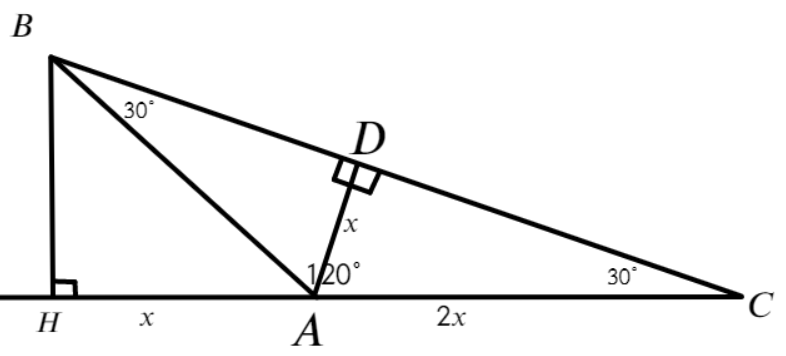
\includegraphics[scale=0.35]{g66.png}}
\end{figure}\\
Чтобы найти расстояние от $A$ до $BC,$ проведём $AD\perp BC.$ Найдём $\angle C=180^\circ-120^\circ-30^\circ=30^\circ,\ \angle BAD=90^\circ-30^\circ=60^\circ, \angle BAH=180^\circ-120^\circ=60^\circ.$ Тогда прямоугольные треугольники $BAD$ и $BAH$ равны по гипотенузе ($AB$ --- общая) и острому углу, а значит $AD=AH.$ Обозначим $AD=x,$ тогда по теореме о катете, лежащем напротив угла в $30^\circ$ для треугольника $ADC,$ имеем $AC=2x.$ Таким образом, $HC=AH+AC=x+2x=3x=12$см, откуда $AD=x=4$см.\\
